\documentclass[12pt]{report}
\usepackage[utf8]{inputenc}
\usepackage[a4paper,width=160mm,top=25mm,bottom=25mm]{geometry}
\usepackage[hyphens]{url}
\usepackage{lipsum}
\usepackage{graphicx}
\usepackage[utf8]{inputenc}
\usepackage[T1]{fontenc}
\usepackage[french]{babel}
\usepackage{acro}
\usepackage{float}
\DeclareAcronym{rdf}{
short = RDF ,
long = Resource Description Framework ,
class  = abbrev
}

\DeclareAcronym{rdfs}{
short = RDFS ,
long = Resource Description Framework Schema ,
class  = abbrev
}

\DeclareAcronym{lod}{
short = LOD ,
long = Linked Open Data ,
class  = abbrev
}

\DeclareAcronym{crdt}{
short = CRDT ,
long =  Conflict-free Replicated Data Type ,
class  = abbrev
}

\begin{document}


\pagenumbering{gobble}
%\input{cover}
%\input{aknowledgment}
\input{abstract}
\listoffigures
\listoftables
\pagebreak
{\large
\printacronyms[include-classes=abbrev,name=Liste des abréviations]}
\tableofcontents
\pagenumbering{arabic}
\chapter*{Introduction Générale}
\addcontentsline{toc}{chapter}{Introduction Générale} \markboth{INTRODUCTION}{}
Dans le Web sémantique et dans le Web en général, un problème fondamental est la comparaison et l’appariement des données et la capacité de résoudre la multiplicité des références de données aux mêmes objets du monde réel, en définissant les correspondances entre les données sous forme de liens de données. La tâche de couplage de données devient de plus en plus importante à mesure que le nombre de données structurées et semi-structurées disponibles sur le Web augmente.
La transformation du Web d’un « Web de documents » en un « Web de données », ainsi que la disponibilité d’importantes collections de données générées par des capteurs (Internet des objets), mènent à une nouvelle génération d’applications Web fondées sur l’intégration des données et des services. Parallèlement, de nouvelles données sont publiées chaque jour à partir de contenus générés par les utilisateurs et de sites Web publics. mène à une nouvelle génération d’applications Web En termes généraux, le couplage de données est la tâche de déterminer si deux descriptions d’objets peuvent être liées l’une à l’autre pour représenter le fait qu’elles se réfèrent au même objet du monde réel dans un cas décrivant les objets du monde réel à travers des sources de données hétérogènes, en supposant que la similarité entre deux descriptions de données est plus élevée, plus grande est la probabilité que la liaison inclut également la tâche de définir des méthodes, des techniques et des outils (semi-)automatisés pour Dans ce contexte, l’une des initiatives les plus importantes dans le domaine du Web sémantique est le lien entre les grandes collections de données déjà disponibles sur le Web \cite{LDOW}. exemple de données liées montre comment la tâche de liaison de données est cruciale sur le Web de nos jours. les méthodes et les techniques de liaison des données sur le Web sémantique. En outre, il existe d’importants travaux décrivant des domaines de recherche très proches des caractéristiques de liaison de données sémantiques qui nécessitent des solutions spécifiques tant en termes de nouvelles techniques que dans Par exemple, d’une part, le couplage de données nécessite de traiter la complexité sémantique typique du couplage ontologique, mais d’autre part, la grande quantité de données disponibles du champ de couplage de données sur le Web sémantique. Dans ce document, nous donnons une définition générale de ce domaine, afin de souligner les problèmes et de décrire les solutions. Nous allons mieux définir le problème de liaison de données, en discutant également de nombreux algorithmes. L’objectif de ce projet est d’étudier les approches existantes en matière d’édition collaborative des données sémantiques, afin de faire une comparaison collaborative entre ces approches, et de proposer un éditeur collaboratif distribué pour les données sémantiques capables de supporter des groupes dynamiques où les utilisateurs peuvent se joindre et partir à tout moment.\cite{WLD}
\chapter{Web et données sémantique}
Le Web sémantique Pour bien comprendre , nous commençons par une définition. Le grand dictionnaire terminologique définit le terme sémantique comme « l'ensemble des relations entre les caractères, ou groupes de caractères, et leur significations, indépendamment de la façon de les employer ou de les interpréter. » Il précise par la suite que « si, en linguistique, la sémantique porte sur l'étude du sens à partir de la combinaison des mots, en intelligence artificielle, elle porte sur la capacité d'un réseau [le Web] à représenter de la manière la plus humaine possible des relations entre des objets, des idées ou des situations. » Le terme sémantique implique donc que la machine ne se contentera plus de présenter visuellement les données du Web, mais, en les reliant, elle pourra conserver les significations qui leur sont attribuables. Or, en transformant le contenu du Web pour qu'il soit « compréhensible » par la machine et non seulement présentable, nous permettons à cette même machine d'être plus efficace dans le traitement de l'information. Ainsi, le dialogue avec les moteurs de recherche devient possible. Nous sommes alors en mesure de nous exprimer dans des termes que nos ordinateurs peuvent aussi interpréter et échanger. Il est également possible  d'automatiser, d'intégrer et de réutiliser l'information entre diverses applicationsLe Web sémantique est décrit généralement comme un Web destiné aux machines. Disposer d'un Web dont le contenu est abordable par les machines peut apporter de grands bénéfices: L'automatisation de nombreuses tâches fondées sur le contenu comme la recherche de ressources ayant un contenu particulier, la comparaison du contenu de ressources (pages, bases de données, ontologies, etc…). Le Web sémantique permettrait de résoudre la relative difficulté de trouver de l'information sur le
web.\cite{SEMANTCWEB}
Le Web sémantique a pour objectif de transformer le World Wide Web actuel, entièrement tourné vers la présentation des 
documents, vers un Web dont le contenu serait compréhensible par les machines. La vision s’appuie sur l’utilisation d’ontologies.
Le Web sémantique n’est pas un Web séparé mais une extension du Web actuel, dans lequel l’information est bien définie, permettant ainsi aux ordinateurs et aux personnes de travailler en coopération.
Le Web sémantique permettra aux machines de comprendre les documents et les données sémantiques, et non la parole humaine et les écrits.\cite{SEMANTCWEB}
\section{\acs{rdf}}
\acs{rdf} est un acronyme de Resource Description Framework. \acs{rdf} est une norme W3C des technologies Web sémantiques et la base de l’architecture standardisée des technologies Web Sémantique. Le \acs{rdf} est un langage simple pour exprimer des modèles de données sous forme d'objets « ressources » et de leurs relations.
Le \acs{rdf} est un langage simple pour exprimer des
modèles de données sous forme d'objets « ressources » et de leurs relations. Il sera utilisé pour annoter des documents écrits
dans des langages non structurés, ou comme une interface pour des documents écrits dans des langages ayant une
sémantique équivalente (des bases de données, par exemple).
Un document \acs{rdf} est un ensemble de triplets de la forme <sujet, prédicat, objet>. Les éléments de ces triplets peuvent être
des URIs (Universal Resource Identifiers), des littéraux ou des variables. Cet ensemble de triplets peut être représenté de façon
naturelle par un graphe (plus précisément un multi-graphe orienté étiqueté), où les éléments apparaissant comme sujet ou objet
sont les sommets, et chaque triplet est représenté par un arc dont l’origine est son sujet et la destination son objet .\cite{SEMANTCWEB}
\acs{rdf} (Resource Description Framework), est un standard décrivant :
\begin{itemize}
 \item des ressources, une ressource pouvant être n'importe quoi (personnes, lieux, animaux, documents,
concepts, etc.) ;
\item la description de ces ressources par des attributs et des relations ;
\item le framework contenant un modèle de données, des langages et des syntaxes.
\end{itemize}
\section{\acs{rdfs}}
Le schéma \acs{rdfs} donne véritablement sa sémantique à la description \acs{rdf}\cite{RDFS}
Il permet aussi de définir un vocabulaire pouvant être utilisé pour décrire des
ressources.
On peut imaginer à loisir de nombreux vocabulaires différents, adaptés chacun à
un domaine ou à une application spécifique. Notons que les vocabulaires,
appelés aussi schémas de description, sont eux-mêmes écrits en \acs{rdf}, en
utilisant des balises de l'espace de nom \acs{rdfs}(e.g, rdfs:Class,
rdfs:subClassOf,rdfs:domain, rdfs:range,...). la figure 1 présente un schéma de
description écrits en \acs{rdf}. Deux de vocabulaire sont définis pour ce schéma.
\textbf{\#Personne}, \textbf{\#Chercheur}, \textbf{\#Doctorant} sont des classes de ressources d'un
annuaire universitaire, \textbf{\#Chercheur} et \textbf{\#Doctorant} sont les sous classes de
\textbf{\#Personne}. \textbf{\#nom} et {\#email} sont des propriétés applicables aux ressources de la
classe \textbf{\#Personne} pour donner le nom et l'adresse email de chacune.
\textbf{\#sousDirection} est une propriété d'association entre \textbf{\#Doctorant} et
\textbf{\#Chercheur}. La figure \ref{rdfs_example} illustre un example d'un shema \acs{rdfs}.
\begin{figure}[H]
\centering
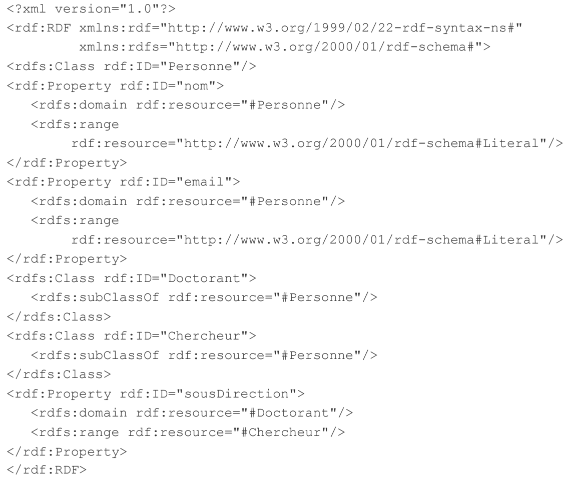
\includegraphics[width=\textwidth]{rdfs_example.png}
\caption{Un schéma de description défini en \acs{rdfs}}\label{rdfs_example}
\end{figure}
\section{LINKED DATA (DONNÉES LIÉES)}
Le Web est de plus en plus considéré comme un espace d’information global constitué non seulement de documents liés, mais aussi de données liées. Plus qu’une simple vision, le Web of Data qui en résulte est né de la maturation de la pile de technologies du Web sémantique et de la publication d’un nombre croissant d’ensembles de données selon les principes des Données Liées
\cite{LDOW}.
\subsection{LINKED OPEN DATA}
Linekd Open Data définit une vision des données liées et accessibles globalement sur l'internet, basée sur
les normes \acs{rdf} du web sémantique. \acs{lod} est souvent considéré comme un nuage de données virtuel où
chacun peut accéder à toutes les données qu'il est autorisé à voir et peut également ajouter à toutes les
données sans perturber la source de données originale. Cela fournit un environnement ouvert où les
données peuvent être créées, connectées et consommées à l'échelle de l'internet. Une théorie de base de
\acs{lod} est que les données ont plus de valeur si elles peuvent être connectées à d'autres données. Dans ce
contexte, les données sont toute information structurée basée sur le web.
Le \acs{lod} a été proposé comme base pour un gouvernement ouvert et pour résoudre de nombreux
problèmes d'intégration de données
\subsubsection{Avantages \acs{lod}:}
En outre, la mise en relation des ensembles de données ouvertes favorise la créativité et l'innovation, car
tous les développeurs, les citoyens et les entreprises peuvent utiliser tous ces ensembles de données pour
mettre les choses en contexte et créer des connaissances et des applications.
Certains des avantages des données ouvertes liées sont :
\begin{itemize}
 \item Utilisation efficace des ressources : Les données ouvertes liées réduisent la redondance en s'appuyant sur
le travail des autres plutôt que de reproduire les systèmes existants.
\item Amélioration de la qualité des informations : Les données ouvertes liées encouragent la normalisation des
métadonnées et des formats de données, ce qui rend les données plus fiables et crédibles.
\item Création de valeur ajoutée : En se connectant directement à d'autres données, les données ouvertes liées
permettent aux utilisateurs de découvrir, d'utiliser et de réutiliser les informations de manière nouvelle et
inattendue.
\item Identification des lacunes dans les informations : Les données ouvertes liées permettent de mettre en
évidence et de corriger les erreurs de données.
\item Amélioration de la transparence : Les données ouvertes liées créent les moyens pour les citoyens et les
groupes de défense de demander des comptes au secteur privé et aux gouvernements.
\end{itemize}

\section{Edition des données sémantiques}
Le développement fulgurant du Web 2.0 est à l’origine d’une nouvelle génération des éditeurs appelés 'éditeurs collaboratifs' passant de la centralisation à la décentralisation et de l’individu à la communauté. Depuis son introduction, le type de données répliqué commutatif (\acs{crdt}) a été largement étudié et continue d'être l'objet de nombreux travaux de recherche. Cet ouvrage présente la conception d’une nouvelle approche originale destinée à la réplication optimiste pour l’édition collaborative des stores sémantiques sur réseaux P2P. L’idée principale de ce travail est de concevoir un nouveau type de données commun et réplicatif pour les entrepôts sémantiques qui dépasse les limites d’un éditeur centré sur une architecture client/serveur à une architecture dynamique P2P, et cela afin de supporter la construction des connaissances de façon collaborative, de supporter le passage à l’échelle en termes d’utilisateurs et ressources, de supporter la dynamicité des pairs et d’assurer la disponibilité des triples-stores \cite{EDIT}.
edition des données semantique.txt
Displaying edition des données semantique.txt.
\section{\acs{crdt} (type de donnée répliqué commutatif)}
C'est un type de données répliqué pour lequel certaines propriétés mathématiques simples garantissent une cohérence
éventuelle. Dans l’État style, les états successifs d’un objet devraient former un semi-réseau monotone, avec fusionner le calcul
d’une limite inférieure. Dans le style op-based, concurrent En supposant seulement que le sous-système de communication
assure la livraison éventuelle (en ordre causal pour les objets basés sur les opérations), les \acs{crdt} sont garantie de converger
vers un état commun et correct, sans nécessiter synchronisation.
L'idée principale est de trouver le type de données pour les déplacements naturels
Partant de ce principe, tout type de \acs{crdt} a été démontré dans Convergence si toutes les opérations sont référencées par des
identifiants uniques différent Le défi se résume donc à concevoir des types de données et des techniques approprié pour
assurer la commutativité des opérations.
\cite{CRDT}
L'idée consiste à associer un identifiant unique à chaque emplacement partagez des symboles , des lignes ou des atomes des
documents . Si l’operation est généré, l'identifiant unique est également associé au paramètre positionelle Cependant, la
gestion des identifiants est un problème très sérieux car La précision de cette méthode repose sur l'unicité et la préservation de
l'identifiant Un changement dans l'ordre général des opérations. Par conséquent, la plage de valeurs de l'identifiant doit être
choisie pour être compacte. Ainsi, entre les deux identifiants Etant donné, il doit toujours être possible de créer un nouvel
identifiant.
Parmi les algorithmes de \acs{crdt} existants, nous distinguons : OR-Set , C-SET ,SU-Set , B-SET, sr-CE et LD-SET Nous
présentons ci-après chacun de ces algorithmes.
\begin{table}[h]
\caption{Par exemple : Soit la phrase simple suivante : la tour Eiffel est créée en 1887 a paris .
Cette phrase est composée des parties suivantes}
\label{table:crdt-example}
\centering
\begin{tabular}{|l|l|}
\hline
Sujet (ressource)    & Tour Eiffel  \\ \hline
Prédicat (propriété) & Créée/située \\ \hline
Objet (littéral)     & 1887/ Paris  \\ \hline
\end{tabular}
\end{table}
\section{Les algorithmes d'édition de données sémantique}
\subsection{OR-Set}
OR-Set est conçu pour la mise à jour basée sur les éléments, il n’est pas adapté pour les opérations basées sur les modèles comme les opérations de mise à jour SPARQ  Afin de réduire la complexité de la communication, au lieu d’étiqueter chaque élément séparément Remarquez que dans le cas d’OR-Set, le nombre de tours serait égal à le nombre de triples exploités, car nous devons envoyer un message pour chaque un. Les triples en double n’affectent pas la complexité des tours, ils sont traités comme un insertion normale.
\subsection{C-SET \cite{C-SET}}
est un \acs{crdt} conçu pour le type de données de l’ensemble.
compteur associé à chaque élément pour garder une trace du nombre de fois qu’il a été ajouté et supprimé. Un élément est considéré comme membre du C-Set si son compteur
est supérieur à zéro. C-Set est convergent, laisse la causalité au sous-jacent réseau, mais malheureusement, quand une suppression suivie d’un insert sont exécutés
l’intention n’est pas préservée. La figure 4 présente un exemple de violation de l’intention dans l’ensemble C. À partir d’un point où un élément x a 3 dans son compteur et donc, pas un membre de l’ensemble. Si deux nœuds décident simultanément pour insérer x et le supprimer immédiatement, ils convergeront vers un état où x est un membre de l’ensemble, ce qui n’était l’intention d’aucun d’eux.
\subsection{SU-Set}
SU-Set a été développée pour servir comme une base pour les entrepôts \acs{rdf} qui 
pourrait s’implémenter dans un moteur d’inférence \acs{rdf}. SU-Set modifie le comportement des 
opérations à diffuser de telles sortes que l’ensemble des triplets seront affectés un par un.
\subsection{B-SET \cite{B-SET}} repose sur l’entreposage de « pierres tombales », c.-à-d. les éléments supprimés sont simplement cachés à l’utilisateur via l’opération de recherche. L’utilisation de pierres tombales n’est pas appropriée pour les grands ensembles comme ceux que nous pouvons trouver dans le réseau de données, car leur complexité spatiale est élevée.
\subsection{srCE}
Une importante propriété du modèle srCE est que ses opérations ne s’exécutent pas 
directement sur l’ensemble final mais elles doivent d’abord s’exécuter sur l’un des multi-sets 
supplémentaires, selon le type de l’opération. Par la suite, une opération interne se génère en vue 
de produire un ensemble cohérent.
\subsection{LD-SET}
LD-Set est conforme à \acs{crdt}, il garantit la cohérence éventuelle dans tout les cas LD-Set concentre sur un mécanisme de réplication optimiste. Il vise à
soutenir l’édition collaborative sociale de Données liées au sein d’une communauté virtuelle d’utilisateurs de différents sites, tout en maintenant une cohérence éventuelle afin de mise à jour simultanée

\subsection{Le modèle CCI :}
Dans le contexte de l’édition collaborative, un système d’édition collaborative partageant des
données répliquées est considéré comme correct s’il assure un modèle de cohérence, plus
précisément le modèle de CCI qui garantit à la fois la convergence des répliques et
préserve la causalité et l’intention de toute opération générée dans le système.
\section{Etude comparative entre ces algorithmes}

SrCE est une approche destinée à la réplication optimiste pour l’édition collaborative des stores
sémantiques sur un réseau P2P.
Un réseau P2P est une collection de machines, appelées appepaires , qui échangentdes données via un
système de communication. La spécificité est que ces machines peuvent à la fois être client et/ou serveur.
C-Set aussi assure la convergence mais ne mentionne pas la garantir des critères de causalité, de cohérence et de préservation de l'intention du modèle CCI.
B-Set est conçu non seulement pour assurer la convergence des répliques triples mais aussi pour
préserver les intentions de l'utilisateur intégrées dans une architecture distribuée. Les ensembles
d'opérations sont également définis afin de permettre l'édition simultanée des mêmes mémoires triples
partagées.
SU-set permet d'assurer la causalité, la convergence et les intentions dans une vision d'un "Live" Linked
Data.
LD-Set se concentre sur un mécanisme de réplication optimiste. Elle vise à
l'édition collaborative sociale de données liées distribuées au sein d'une communauté virtuelle
d'utilisateurs de différents sites, tout en maintenant une cohérence éventuelle afin de permettre
mise à jour simultanée.
apres avoir certaints algorithmes de \acs{crdt} nous terminons notre étude comparative par \ref{table:comp} qui
résume une comparaison entre eux

\begin{table}[]
\caption{Résumé de comparaison entre les algorithmes}
\label{table:comp}
\begin{tabular}{lcccccc}
CCI         & \multicolumn{1}{l}{B-set} & \multicolumn{1}{l}{C-Set} & \multicolumn{1}{l}{SU-Set} & \multicolumn{1}{l}{LD-Set} & \multicolumn{1}{l}{Or-Set} & \multicolumn{1}{l}{SrCE} \\
causalité   &                           & -                         &                            &                            &                            &                          \\
cohérence   &                           & -                         & -                          & X                          &                            & X                        \\
l'intention & X                         & -                         & X                          &                            &                            & X                        \\
convergence & X                         & X                         & X                          & X                          & X                          & X                       
\end{tabular}
\end{table}

\section*{Conclusion}
Dans ce chapitre, nous avons présenté le web semantique, linked data et quelques modèles d’édition collaboratifs basés sur l’approche des
\acs{crdt}. nous avons évalué les algorithmes \acs{crdt} étudiés dans ce chapitre selon le modèle CCI. Malgré leur robustesse elles ont leurs faiblesses. Par conséquent, dans le chapitre suivant, nous travaillerons sur l'amélioration de l'un des algorithmes susmentionnés.
\addcontentsline{toc}{chapter}{Conclusion} \markboth{CONCLUSION}{}

\bibliography{bibio} 
\bibliographystyle{ieeetr}
\end{document}
